% IEEE Signal Processing Letters submission
% Compile: see ../README.md (python make_numbers.py; pdflatex; bibtex; pdflatex x2)
\documentclass[journal]{IEEEtran}

\usepackage[T1]{fontenc}
\usepackage{amsmath,amssymb,amsfonts}
\usepackage{amsthm}
\usepackage{graphicx}
\usepackage{booktabs}
\usepackage{cite}
\usepackage[hidelinks]{hyperref}

\graphicspath{{../figures/}}
% auto-generated by make_numbers.py -- do not edit
\newcommand{\delayBoundN}{16}
\newcommand{\delayExcess}{0.11}
\newcommand{\delayOverhead}{1.0}
\newcommand{\nSeeds}{3}
\newcommand{\aucAtKmin}{0.69}
\newcommand{\aucAtKmax}{0.72}
\newcommand{\ratioLTIa}{2.0}
\newcommand{\ratioSela}{2.0}
\newcommand{\ratioLTIb}{2.7}
\newcommand{\ratioSelb}{2.7}
\newcommand{\ratioLTIc}{4.0}
\newcommand{\ratioSelc}{3.3}
\newcommand{\ratioLTId}{4.0}
\newcommand{\ratioSeld}{5.1}
\newcommand{\belowN}{22}
\newcommand{\belowUnderLTI}{22}
\newcommand{\belowUnderSel}{22}
\newcommand{\leakLo}{0.49}
\newcommand{\leakHi}{0.52}
\newcommand{\selDiff}{$-0.001$}
\newcommand{\selCI}{0.002}
\newcommand{\selP}{0.005}
\newcommand{\dtCV}{1}
\newcommand{\shiftAtK}{0.59}
\newcommand{\shiftAtKp}{1.00}
\newcommand{\frozenAtK}{0.87}
\newcommand{\frozenAtTwoK}{0.97}
\newcommand{\ltiAtK}{0.70}
\newcommand{\ltiAtTwoK}{0.85}
\newcommand{\ltiEightThirtyTwo}{0.99}
\newcommand{\nocmpEightThirtyTwo}{0.99}
\newcommand{\nocmpMaxDiff}{0.02}
\newcommand{\frozenKlo}{0.92}
\newcommand{\frozenKhi}{0.97}
\newcommand{\frozenSixteen}{0.64}
\newcommand{\frozenSixteenCI}{0.26}
\newcommand{\shiftAtKlo}{0.51}
\newcommand{\shiftAtKhi}{0.62}
\newcommand{\cslSmax}{64}
\newcommand{\cslLTIatTwo}{24.0}
\newcommand{\cslOrBest}{98.3}
\newcommand{\cslLTIBest}{60.4}
\newcommand{\cslLTIBestCI}{7.9}
\newcommand{\cslSelBest}{55.2}
\newcommand{\cslSelBestCI}{8.5}
\newcommand{\cslAuxBest}{56.2}
\newcommand{\cslAuxBestCI}{13.7}
\newcommand{\cslAuxBestS}{64}
\newcommand{\cslLTIatAuxS}{60.4}
\newcommand{\cslSelMinusLTI}{$-1.7$}
\newcommand{\cslSelMinusLTICI}{1.1}
\newcommand{\cslEvalLenGain}{1.9}
\newcommand{\poolTwoOne}{53.7}
\newcommand{\poolTwoSixteen}{86.3}
\newcommand{\cslWmin}{3}
\newcommand{\cslWmax}{8}
\newcommand{\cslGridOr}{10}


\newtheorem{theorem}{Theorem}
\newtheorem{proposition}{Proposition}
\newtheorem{corollary}{Corollary}
\theoremstyle{remark}
\newtheorem{remark}{Remark}

\newcommand{\R}{\mathbb{R}}
\newcommand{\E}{\mathbb{E}}
\newcommand{\one}{\mathbf{1}}
\newcommand{\Hk}{\mathcal{H}_k}
\DeclareMathOperator{\rank}{rank}

\begin{document}

\title{Hankel-Norm and Information Limits on Delay Detection by Low-Order
State-Space Models, with Application to Graph Random Walks}

\author{Olivia~Kim and Aryan~Padarthi%
\thanks{Manuscript received XX; revised XX. The associate editor coordinating the review of this manuscript and approving it for publication was XX.}%
\thanks{The authors are with the Allen Independent School District, Allen, TX, USA (e-mail: olivia.kim@student.allenisd.org; aryan.padarthi@student.allenisd.org).}%
\thanks{Code and data: \url{https://github.com/The-MathKing/ITE}.}}

\markboth{IEEE Signal Processing Letters,~Vol.~XX, 2026}%
{Kim and Padarthi: Limits on Delay Detection by Low-Order State-Space Models}

\maketitle

\begin{abstract}
An order-$S$ linear time-invariant (LTI) state-space model reads a sequence
and must decide whether the current sample repeats the one $k$ steps
earlier. This delay-and-compare primitive underlies cycle detection by
random-walk graph learners. We show that exact detection requires $S\ge k+1$
and a nilpotent (FIR) state matrix, and is impossible at every $S$ for
invertible dynamics such as S4D and Mamba. Because the lag-$k$ delay has $k$
unit Hankel singular values, for $S<k$ no linear probe improves on the zero
probe in Hankel norm, and any probe explains at most a fraction $S/k$ of the
delayed sample's variance. For Gaussian inputs this bounds every nonlinear
readout, with detection divergence at most $\tfrac12\ln\frac{k}{k-S}$.
Optimal fits follow the $S/k$ law, a trained shift register switches on
exactly at $S=k+1$, and trained diagonal SSMs stay below the Gaussian ceiling
but need \ratioLTIc$\times$ the minimal state to reach an AUROC of $0.95$. On
circular skip-link graphs, non-backtracking return horizons predict when
exact-count features separate classes.
\end{abstract}

\begin{IEEEkeywords}
State-space models, Hankel operators, model order reduction, detection, random walks on graphs.
\end{IEEEkeywords}

\section{Introduction}
\IEEEPARstart{D}{eciding} whether a signal repeats itself after a lag $k$ is
a basic detection task: it is echo detection, and it is the primitive that
sequence models must implement to recall earlier inputs. Structured
state-space models (SSMs)~\cite{gu2022s4,gu2022s4d,gu2024mamba} implement it
with a recursive filter of order $S$, and much of their design is about
approximating delays with few states~\cite{voelker2019lmu,gu2020hippo}. That
the pure delay $z^{-k}$ has McMillan degree $k$ is classical realisation
theory~\cite{ho1966kalman,glover1984hankel,aak1971}. What is missing is a
\emph{rate}: how much of the delayed sample can an order-$S$ state carry when
$S<k$, and what does that imply for detection by an arbitrary nonlinear
readout? Related limits for recurrent models concern memory decay and
optimisation~\cite{li2021curse}, copying and associative
recall~\cite{jelassi2024repeat,arora2024zoology}, and state
tracking~\cite{merrill2024illusion}.

Our application is graph learning. Message-passing GNNs are bounded by the
1-WL test~\cite{xu2019gin,morris2019wl} and cannot separate the regular
circular skip-link (CSL) graphs~\cite{murphy2019rp,dwivedi2023benchmarking}.
Walk-based learners read random walks as
sequences~\cite{toenshoff2023crawl,chen2025neuralwalker,kim2025rwnn}, and
random node features~\cite{abboud2021rni,sato2021rf} turn walk revisits,
and hence closed walks, into token repetitions. SSMs are now used as the
sequence backbone of such models~\cite{wang2024graphmamba,behrouz2024graphmamba,chen2025neuralwalker}.

Our contributions are:
(i) \emph{exact limits}: exact lag-$k$ detection needs $S\ge k+1$ with
nilpotent dynamics and is impossible for invertible dynamics at any $S$;
(ii) \emph{rates}: for $S<k$, no linear probe beats the zero probe in Hankel
norm, the explained variance is at most $S/k$, and for Gaussian inputs this
bounds the divergence available to every readout;
(iii) \emph{graph consequence}: exact non-backtracking (NB) return horizons
$W^*(r)$ at which window features separate each CSL class; and
(iv) \emph{validation}: optimal fits, a shift-register control, frozen fitted
poles and seeded experiments that separate the information limit from the
optimisation overhead of trained SSMs.

\section{Problem Setting}
A sequence model with real state $s_t\in\R^S$ reads tokens $x_t\in\R^d$:
\begin{equation}
  s_t = A_t s_{t-1} + B_t x_t,\qquad \hat y_t = g(s_t,x_t),
  \label{eq:ssm}
\end{equation}
with an arbitrary readout $g$. It is \emph{LTI} if $A_t\equiv A$ and
$B_t\equiv B$. The \emph{lag-$k$ repeat} label is $y_t=\one[x_t=x_{t-k}]$.
In the graph setting, $v_0,v_1,\dots$ is an NB walk ($v_{t+1}\ne v_{t-1}$),
each walk draws fresh features $f_v\sim\mathcal N(0,I_d)$ i.i.d.\ over nodes,
and $x_t=f_{v_t}$. Then $y_t=\one[v_t=v_{t-k}]$ almost surely, i.e.\ $y_t=1$
exactly when the last $k$ steps form a closed NB walk. Their frequencies
follow from powers of the Hashimoto (NB) operator~\cite{hashimoto1989zeta,alon2007nbw}.

\section{Limits}
\begin{proposition}[Exact detection]\label{prop:exact}
Let $(A,B)$ be LTI and $g$ arbitrary. (a) If $S\le k$, or (b) if $A$ is
invertible (any $S$), then there are two token sequences with the same
$(s_t,x_t)$ and $y_t=1$, $y'_t=0$. (c) If $S\ge k+1$, the shift register
$s_t=(w^\top x_t,\dots,w^\top x_{t-S+1})$, which has nilpotent $A$, detects
$y_t$ exactly for almost every $w$.
\end{proposition}
\begin{IEEEproof}
Fix $\eta\ne0$ and let $p(\lambda)=\sum_{i\le q}p_i\lambda^i$ be the minimal
polynomial of $A$ on the Krylov space of $B\eta$, so $q\le S$. Any polynomial
$\pi(\lambda)=\sum_{j\ge1}\pi_j\lambda^j$ with $\pi(A)B\eta=0$ and $\pi_k\ne0$
gives a confusable pair. Take a sequence with $x_{t-k}=x_t$ and set
$x'_{t-j}=x_{t-j}+(\pi_j/\pi_k)\eta$ for $j\ge1$. Then
$s_t-s'_t=-\pi_k^{-1}\pi(A)B\eta=0$ and $x'_{t-k}\ne x_t$. (a) If $q<k$, take
$\pi=\lambda^{k-q}p$. If $q=k$ and $p=\lambda^k$, take $\pi=\lambda^k$.
Otherwise let $i<k$ be the largest index with $p_i\ne0$ and take
$\pi=\lambda^{k-i}p$. (b) If $A$ is invertible then $p_0\ne0$; take
$\pi=\lambda^kp$. (c) The register holds $w^\top x_{t-k}$, and for
continuous features $w^\top x_t=w^\top x_{t-k}$ iff $x_t=x_{t-k}$ almost surely.
\end{IEEEproof}

Every S4D or Mamba discretisation $A=\exp(\Delta\Lambda)$ is invertible, so
exactness is never available to them. The relevant question is how
\emph{well} an order-$S$ state can carry the lag-$k$ sample. A linear
probe $z_t=c^\top s_t+\beta^\top x_t$ estimates $w^\top x_{t-k}$ with
$\|w\|=1$. Its error $z_t-w^\top x_{t-k}=\sum_{m\ge0}e_mx_{t-m}$ has taps
$e_m=c^\top A^mB-\delta_{m,k}w^\top$ for $m\ge1$ and transfer function
$E(z)=\sum_{m\ge1}e_mz^{-m}$, with $\|E(e^{j\omega})\|$ the Euclidean norm of
the $1\times d$ row. Let $\Hk(f)$ be the $k\times kd$ block-Hankel section
with $(i,j)$ block $f_{i+j+1}$, $0\le i,j<k$.

\begin{theorem}[Hankel limits]\label{thm:hankel}
If $S<k$, every LTI probe satisfies
\begin{align}
 &\|\Hk(e)\|_2\ \ge\ 1,\quad\text{hence}\quad \textstyle\sup_\omega\|E(e^{j\omega})\|\ \ge\ 1, \label{eq:hinf}\\
 &\|\Hk(e)\|_F^2=\textstyle\sum_{m=1}^{2k-1}\min(m,2k-m)\|e_m\|^2\ \ge\ k-S. \label{eq:frob}
\end{align}
Hence, for i.i.d.\ unit-variance tokens,
$\E[(z_t-w^\top x_{t-k})^2]\ge1-S/k$: the probe explains at most a fraction
$S/k$ of the variance. For $S=k$ the infimum of the error is $0$, but it is
not attained.
\end{theorem}
\begin{IEEEproof}
Since $h_{i+j+1}=(c^\top A^i)(A^{j+1}B)$, we have $\rank\Hk(h)\le S$. The
target $\delta_{m,k}w^\top$ gives a block anti-diagonal matrix with $k$ unit
singular values. Eckart--Young--Mirsky~\cite{eckart1936} in the spectral and
Frobenius norms gives $\|\Hk(e)\|_2\ge\sigma_{S+1}=1$ and
$\|\Hk(e)\|_F^2\ge\sum_{i>S}\sigma_i^2=k-S$. A finite section is bounded by
the Hankel operator, which is a compression of the Laurent operator of $E$;
this gives~\eqref{eq:hinf}, and equality in the limit is Nehari's
theorem~\cite{nehari1957}. The tap $e_m$ occurs $\min(m,2k-m)\le k$ times,
which gives~\eqref{eq:frob} and the variance bound. For $S=k$, take
$A=\gamma P$ with $P$ the $k$-cycle permutation, $B=u_1w^\top$,
$c=\gamma^{-k}u_1$ and $\beta=-\gamma^{-k}w$. Then $e_m=\gamma^{m-k}w^\top$
for $m\in\{2k,3k,\dots\}$ and $0$ otherwise, so the error is
$\gamma^{2k}/(1-\gamma^{2k})\to0$ as $\gamma\to0$.
\end{IEEEproof}

Bound~\eqref{eq:hinf} says that for $S<k$ no LTI probe beats outputting zero
in Hankel norm: all Hankel singular values of $z^{-k}$ equal one, so its
optimal Hankel-norm approximant of degree $<k$ is
zero~\cite{aak1971,glover1984hankel}. Bound~\eqref{eq:frob} is the rate.
Under Gaussian inputs it extends to every readout.

\begin{corollary}[Any readout]\label{cor:gauss}
Let $x_t$ be i.i.d.\ $\mathcal N(0,I_d)$ and $S<k$. For every measurable
$g$, the minimum mean-squared error of $x_{t-k}$ given $(s_t,x_t)$ is at least
$d-S/k$. For $H_1$: $x_t=x_{t-k}$ against $H_0$: $x_t$ fresh, the
observations satisfy $\mathrm{KL}(P_1\|P_0)\le\tfrac12\ln\frac{k}{k-S}$, so no
detector exceeds balanced accuracy
$\tfrac12+\tfrac12\big(\tfrac14\ln\frac{k}{k-S}\big)^{1/2}$.
\end{corollary}
\begin{IEEEproof}
For jointly Gaussian variables the conditional mean is linear. Stacking $d$
probes gives a target with $kd$ unit Hankel singular values, and
\eqref{eq:frob} yields total error $\ge d-S/k$. Next, $(s_t,x_t)$ is a
function of $(s_{t-1},x_t)$. These are independent under $H_0$ and have the
same marginals under $H_1$, so
$\mathrm{KL}=I(s_{t-1};x_{t-k})=-\tfrac12\sum_i\ln(1-\lambda_i)$, where
$\lambda_i$ are the squared canonical correlations. Applying the bound to
$s_{t-1}$ (the same $k\times k$ Hankel count) gives $\sum_i\lambda_i\le S/k$.
By convexity the maximum puts all mass on one $\lambda_i$. Data processing and
Pinsker's inequality complete the proof.
\end{IEEEproof}

\begin{remark}
The bounds limit \emph{precision}, not information. For $S<k$ the state can
still correlate with the lagged sample, so statistics pooled over many
tokens remain informative. The near-optimal realisation at $S=k$ needs gains
$\gamma^{-k}$ and is exponentially ill-conditioned (cf.~\cite{li2021curse}).
Input-dependent $(A_t,B_t)$ break the factorisation used above, so we test
them empirically. On walks, revisits make tokens dependent. Theorem
\ref{thm:hankel}(\ref{eq:hinf}) is distribution-free; the variance and
divergence rates use the i.i.d.\ surrogate, which we check in
Section~\ref{sec:exp}.
\end{remark}

\textit{NB return horizons.} Let $p_G(\ell)=\Pr[v_\ell=v_0]$ for the
stationary NB walk (uniform on directed edges). We compute it exactly from
the Hashimoto operator~\cite{hashimoto1989zeta}. For a family $\{G_r\}$, let
$W^*(r)$ be the smallest $W$ such that
$\max_{\ell\le W}|p_{G_r}(\ell)-p_{G_{r'}}(\ell)|>\tau$ for all $r'\ne r$. It is the shortest window of revisit
frequencies that separates class $r$. For the ten CSL classes ($n=41$,
skips $r\in\{2,3,4,5,6,9,11,12,13,16\}$), $W^*(r)$ ranges from \cslWmin{}
to \cslWmax{} and is unchanged for $\tau\in[10^{-4},3\cdot10^{-3}]$
(Table~\ref{tab:csl}). $W^*$ is a horizon for \emph{exact} access. An
order-$S$ reader with $S<W^*$ still explains up to $S/\ell$ of the
lag-$\ell$ variance, so pooled estimators can succeed below $W^*$ at a
sample cost that grows as $S/W^*$ shrinks.

\section{Experiments}\label{sec:exp}
\textit{Models.} Our learned SSM is one diagonal complex layer with
S4D-Lin initialisation~\cite{gu2022s4d}. It has $\lfloor S/2\rfloor$ complex
modes plus one real mode if $S$ is odd, so its real state dimension is
exactly $S$. The dynamics are $A=\exp(\Delta\Lambda)$ and $B_t=\Delta B$,
with $\Delta$ learned per mode (\emph{LTI}) or set to
$\Delta_t=\mathrm{softplus}(W_\Delta x_t+v_\Delta)$
(\emph{input-dependent step}, the Mamba-style gate). The readout sees
$[\Re s_t,\Im s_t,x_t]$ and comparison features $(Ux_t-Vs_t)^{\odot2}$,
followed by a two-layer MLP. We use $d=8$ features, AdamW with a cosine
schedule, and \nSeeds{} seeds; intervals are 95\% $t$-intervals. All runs are
on CPU, and a script regenerates every number and figure in this letter.

\textit{Delay realisation.} We fit an $S$-state diagonal impulse response
to $\delta_{m,k}$ ($m\ge1$), keeping the best of four restarts
(Fig.~\ref{fig:delay}). All \delayBoundN{} fits with $S<k$ respect
$\|e\|_2\ge\sqrt{1-S/k}$, with a median excess MSE of \delayExcess{} over
the bound. The error first drops to about $0.1$ at a median of
$S=\delayOverhead\,k$, so the rate of Theorem~\ref{thm:hankel} is nearly
attained by direct fitting.

\begin{figure}[!t]
\centering
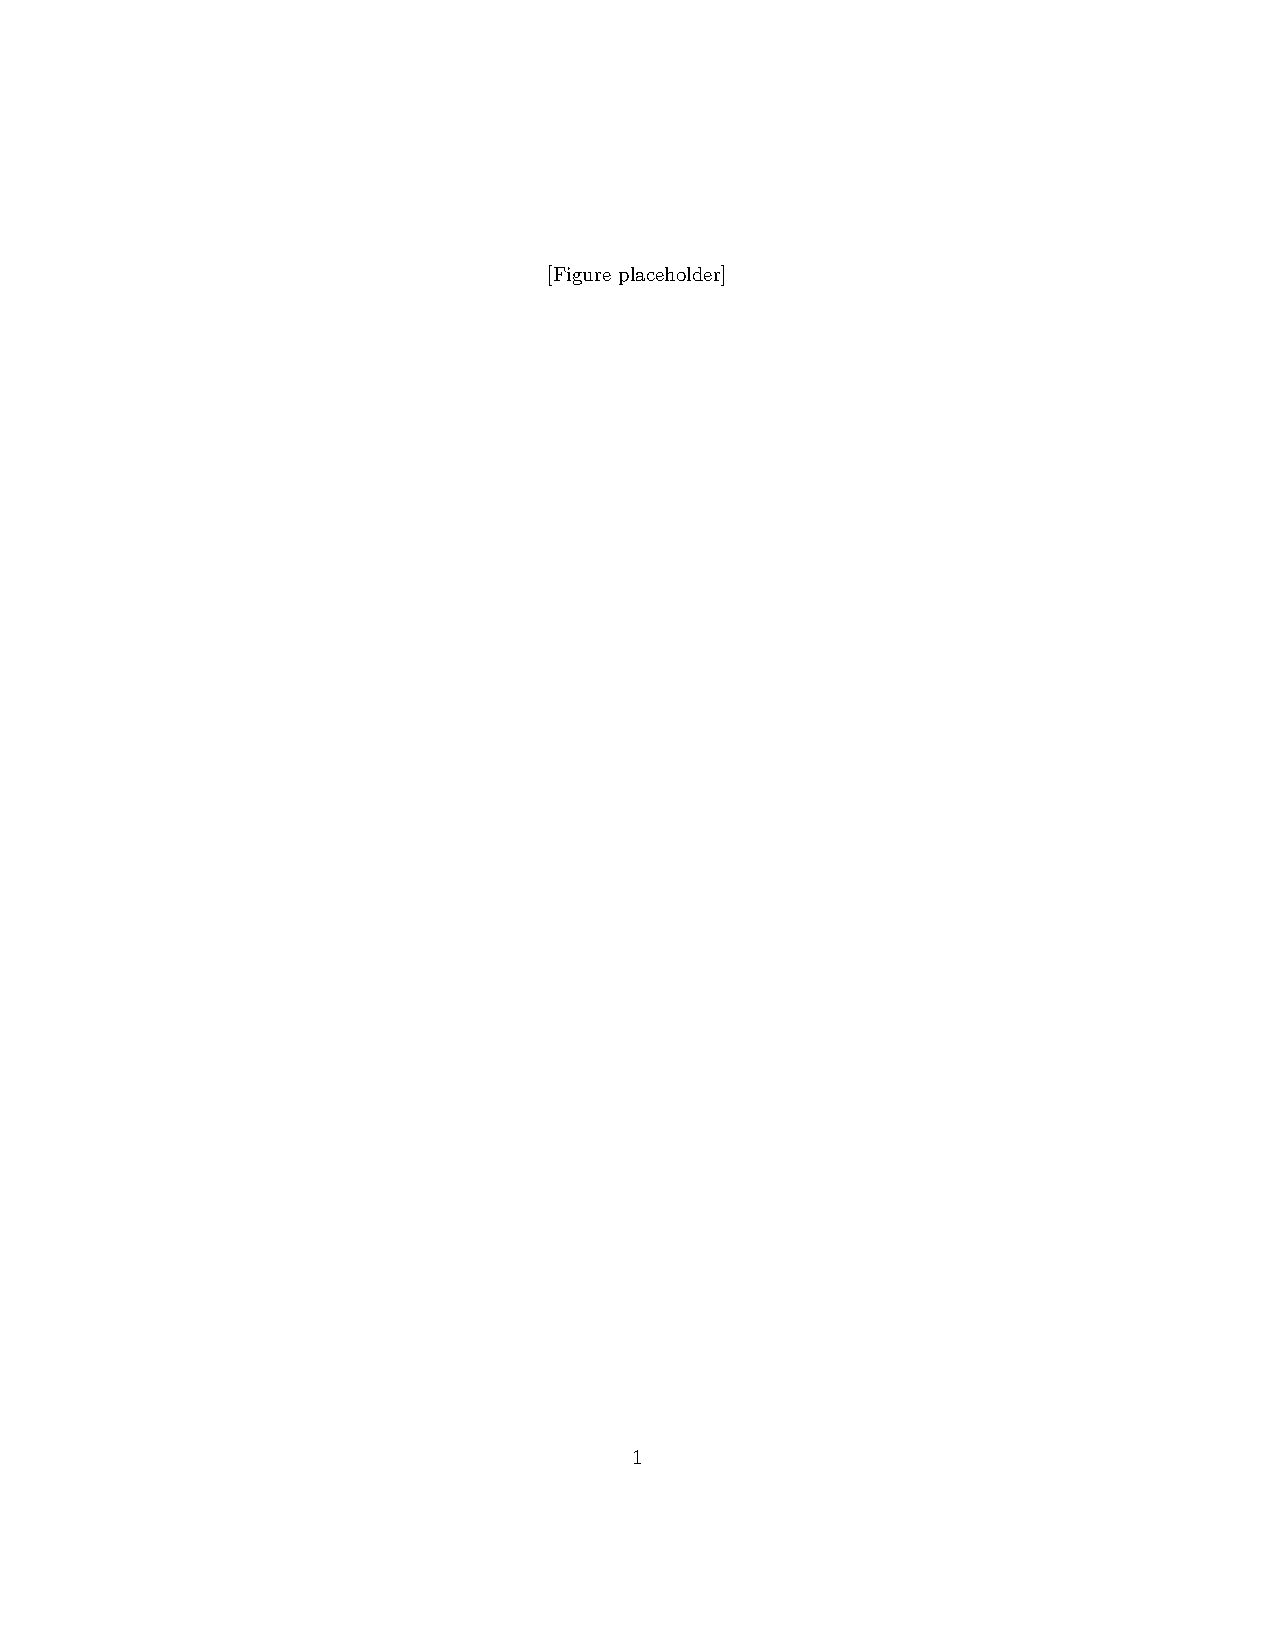
\includegraphics[width=\columnwidth]{fig1_delay_realization.pdf}
\caption{Best gradient fit (four restarts, taps $m\le63$) of an $S$-state
diagonal LTI impulse response to the lag-$k$ delay. Dotted lines: the lower
bound $\sqrt{1-S/k}$ of Theorem~\ref{thm:hankel} for $S<k$.}
\label{fig:delay}
\end{figure}

\textit{Token-level detection.} We train on NB walks ($T=64$) over 256
random 4-regular graphs ($n=24$, unions of two Hamiltonian cycles) and test
on 64 unseen graphs. Fig.~\ref{fig:phase} shows that the test AUROC for
$y_t$ rises smoothly with $S$. There is no sharp transition at $S=k$, where the AUROC is
\aucAtKmin--\aucAtKmax. The state needed for a given AUROC grows
approximately linearly in $k$. Its median ratio to $k$ is \ratioLTIa, \ratioLTIb,
\ratioLTIc{} and \ratioLTId{} at AUROC thresholds $0.8$, $0.9$, $0.95$ and
$0.99$. Below the bound, all \belowN{} LTI cells lie under the optimal AUROC
of the Gaussian surrogate with explained variance $S/k$ (Fig.~\ref{fig:ratio}).
The surrogate is justified on these graphs: a Bayes-optimal table of the exact
revisit indicators at lags $1,\dots,S-1$ predicts lag-$k$ revisits at AUROC
\leakLo--\leakHi, so short-lag walk structure carries no information about
lag-$k$ revisits. The input-dependent step changes the AUROC by
\selDiff$\pm$\selCI{} (mean over cells; Wilcoxon $p=\selP$), and its learned
$\Delta_t$ varies by only \dtCV\% across tokens. Random features give the
gate nothing to select on, so this is expected.

\begin{figure*}[!t]
\centering
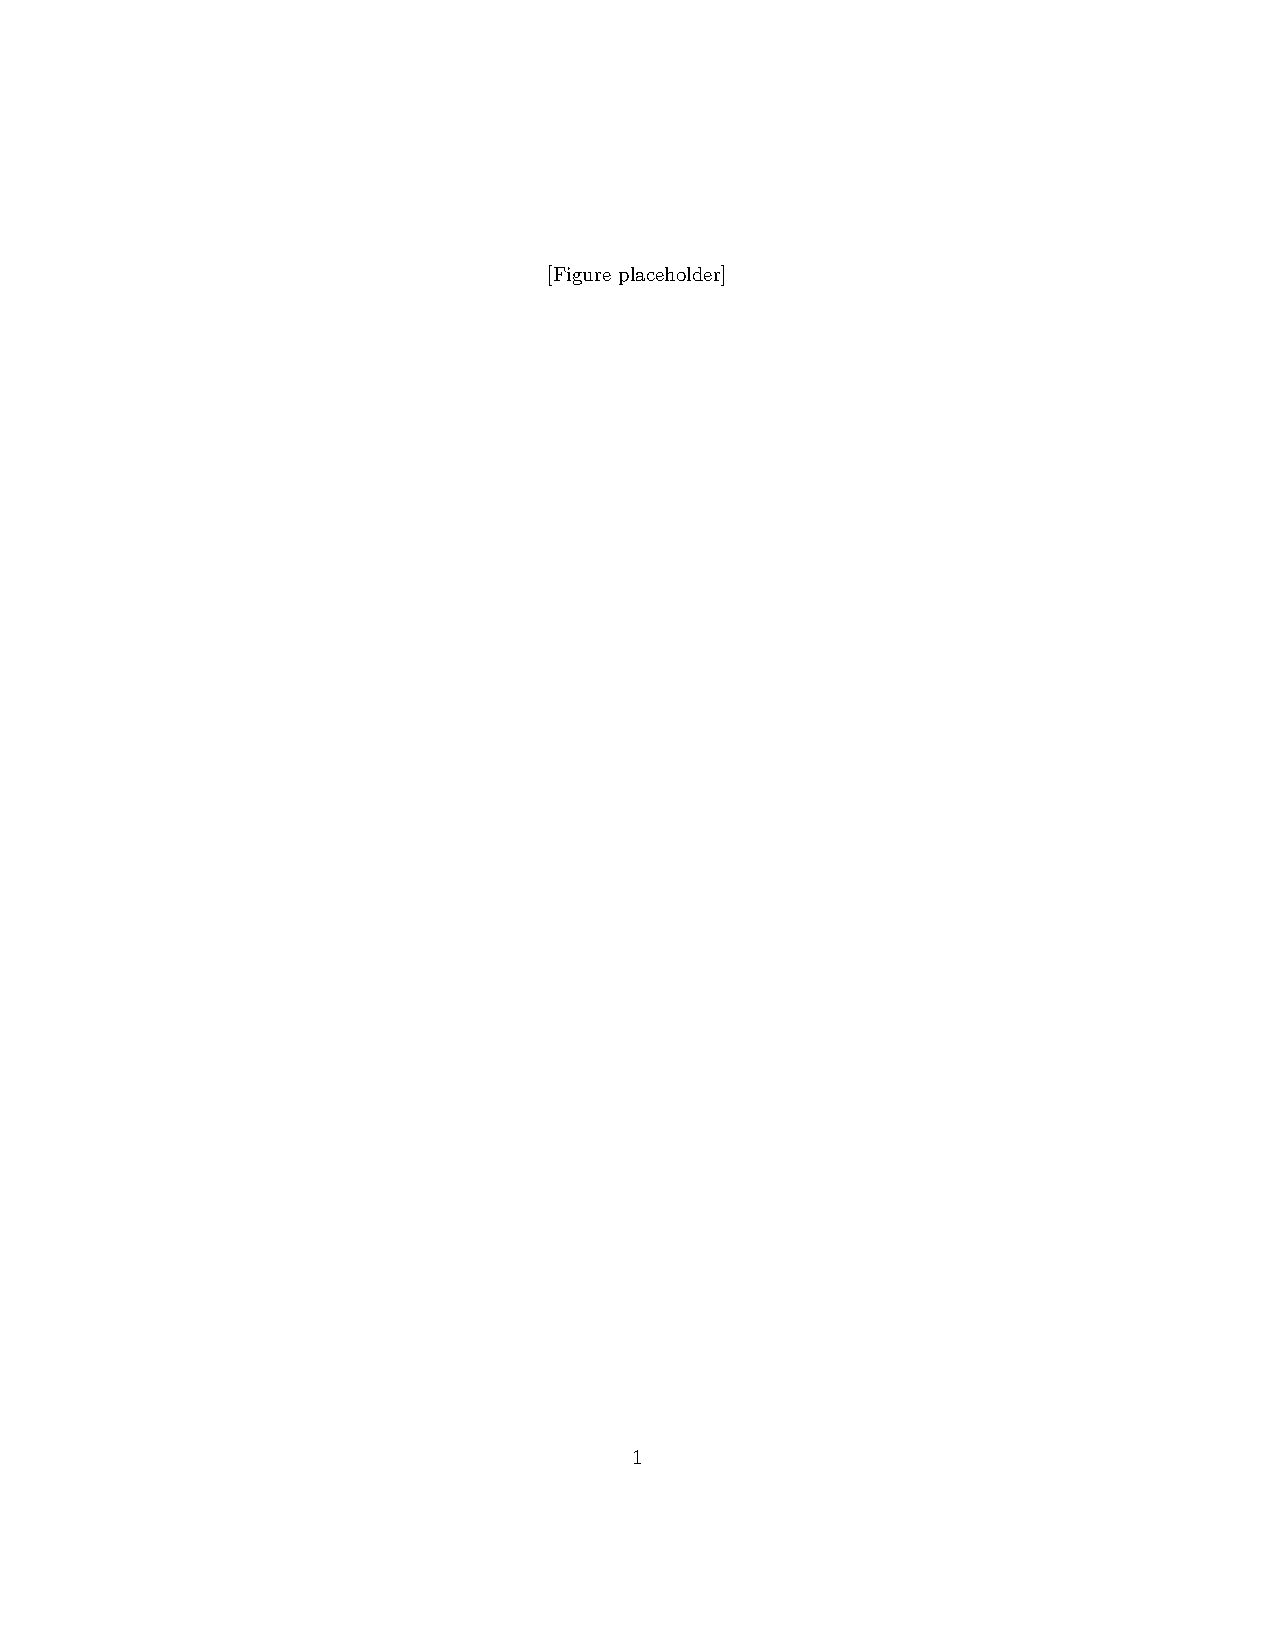
\includegraphics[width=\textwidth]{fig2_phase_diagram.pdf}
\caption{Lag-$k$ revisit detection on NB walks over random 4-regular graphs
($n=24$, $T=64$, $d=8$), mean of \nSeeds{} seeds. (a) Test AUROC of the LTI
model; the dotted line marks the first $S$ with AUROC $\ge0.95$. (b)
Input-dependent step minus LTI. Red dashed line: $S=k$.}
\label{fig:phase}
\end{figure*}

\textit{Controls.} Three controls separate the information limit from
training effects (Fig.~\ref{fig:ratio}).
\begin{itemize}
\item \emph{Shift register.} A trained shift register (nilpotent $A$, learned $w$)
has AUROC \shiftAtK{} at $S=k$ and \shiftAtKp{} at $S=k+1$, the switch predicted
by Proposition~\ref{prop:exact}(c).
\item \emph{Frozen poles.} Freezing the poles at the delay fit of
Fig.~\ref{fig:delay} and training only $B$ and the readout gives \frozenAtK{} at
$S=k$ and \frozenAtTwoK{} at $S=2k$, against \ltiAtK{} and \ltiAtTwoK{} with
learned poles.
\item \emph{Comparison features.} Removing them lowers the $k=8$ AUROC at $S=32$
from \ltiEightThirtyTwo{} to \nocmpEightThirtyTwo.
\end{itemize}
\ControlsInterpretation

\begin{figure}[!t]
\centering
\includegraphics[width=\columnwidth]{fig4_auroc_vs_ratio.pdf}
\caption{Test AUROC against $S/k$ (all $k$, seed means). Solid curve: optimal
AUROC of the i.i.d.\ Gaussian surrogate with explained variance $S/k$
(Corollary~\ref{cor:gauss}). Red dashed line: $S=k$.}
\label{fig:ratio}
\end{figure}

\textit{CSL classification.} CSL graphs are 4-regular and featureless, so
1-WL is provably at chance (10\%). Each training example is one NB walk
($T=128$) on a CSL graph, and the class is predicted from mean-pooled
features. At test time, each graph is judged from 16 walks ($T=256$). As an
\emph{exact-count reference} we use logistic regression on the exact revisit
frequencies at lags $1,\dots,S$. It is not an upper bound. At $S=2$ it is at
chance, because NB walks cannot return at lags 1--2, while the LTI model
reaches \cslLTIatTwo\%. The reference reaches \cslOrBest\%. For all
\cslGridOr{} classes, its onset of 80\% class accuracy is the first tested
$S\ge W^*(r)$ (Table~\ref{tab:csl}). The trained models reach
\cslLTIBest$\pm$\cslLTIBestCI\% (LTI) and \cslSelBest$\pm$\cslSelBestCI\%
(input-dependent step) at $S=\cslSmax$. The largest tested $S$ gives the
best accuracy for both, and the curves are still rising.
\CSLInterpretation{} Class $r=2$ ($W^*=3$) is learned at $S=2$ only by
pooling: with one walk its accuracy is \poolTwoOne\%, and with 16 walks it
is \poolTwoSixteen\%.

\begin{figure}[!t]
\centering
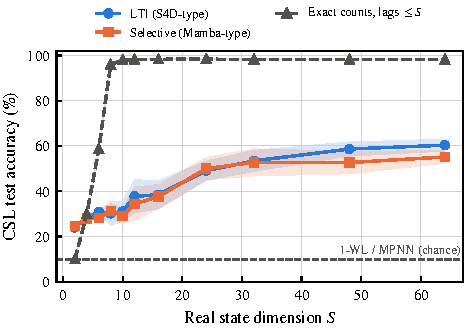
\includegraphics[width=\columnwidth]{fig3_csl_accuracy.pdf}
\caption{CSL test accuracy against $S$ (mean and 95\% interval over
\nSeeds{} seeds; test graphs are the ten CSL graphs with fresh walks and
features). The exact-count reference uses revisit frequencies at lags
$\le S$.}
\label{fig:csl}
\end{figure}

\begin{table}[!t]
\centering
\caption{CSL horizons $W^*(r)$ and per-class onsets: the smallest tested $S$
with class accuracy $\ge80\%$ (mean of \nSeeds{} seeds; ---: not reached for
$S\le\cslSmax$).}
\label{tab:csl}
\setlength{\tabcolsep}{3.2pt}
% auto-generated by make_numbers.py -- do not edit
\begin{tabular}{lcccccccccc}
\toprule
$s$ & 2 & 3 & 4 & 5 & 6 & 9 & 11 & 12 & 13 & 16 \\ \midrule
$W^*(s)$ & 3 & 4 & 5 & 6 & 7 & 8 & 7 & 8 & 5 & 7 \\
Oracle & 4 & 4 & 6 & 6 & 8 & 8 & 8 & 8 & 6 & 8 \\
LTI & 2 & 6 & -- & -- & -- & -- & -- & -- & 32 & -- \\
Selective & 2 & 8 & -- & -- & -- & -- & -- & -- & 64 & -- \\
\bottomrule
\end{tabular}

\end{table}

\section{Conclusion}
The pure delay has $k$ unit Hankel singular values. For an order-$S$ LTI
state this gives three limits: exact detection needs $S\ge k+1$ and
nilpotent dynamics, the explained variance of the lagged sample is at most
$S/k$, and for Gaussian inputs every readout has divergence at most
$\tfrac12\ln\frac{k}{k-S}$. Optimal fits and a shift register attain these
limits. Trained diagonal SSMs respect them, but they need several times the
minimal state, and an input-dependent step does not change this. Lower bounds for
input-dependent dynamics and better-conditioned delay parameterisations are
natural next steps.

\bibliographystyle{IEEEtran}
\bibliography{refs}

\end{document}
